\section{Architektura systemu}

W ramach pracy dyplomowej stworzone zostaną dwa systemy, które za pomocą tej samej techniki komunikacji zrealizują dwa przykładowe zadania, aby zaprezentować możliwości wykorzystania nowo powstałych standardów. Pierwszym z nich jest pilot umożliwiający porusznie kursorem na ekranie komputera pracującego pod systemem Linux lub MacOSX (opisany szczegółowo w sekcji ~\ref{sec:component-controll-remote-screen}). Drugi system to implementacja gry PONG dla dwóch graczy z możliwością kolejkowania kandydatów do gry.


W załączniku ~\ref{app:network_diagram_app} przedstawiono sieć połączeń pomiędzy fizycznymi komponentami architektury. Rysunek pokazuje możliwość skalowalności systemu.


W niniejszej sekcji zostanie przedstawiona architektura systemu w postaci diagramu komponentów oraz interakcji pomiędzy nimi.

\subsection{Pilot do sterowania zdalnym monitorem}

System pilota do sterowania zdalnym monitorem złożony jest z trzech części:

\begin{enumerate}
  \item \textbf{Klienta webowego} w postaci strony internetowej uruchamianej na w przeglądarce internetowej na urządzeniu mobilnym użytkownika końcowego. Jego celem jest:
  \begin{enumerate}
    \item Podłączenie się do serwera za pomocą Web Socket, utrzymywanie połączenia w przeglądarce internetowej.
    \item Przechwytywania gestów wykonywanych na ekranie urządzenia mobilnego oraz translację współrzędnych punktu ich na absolutną, procentową pozycję kursora na płaszczyźnie dwuwymiarowej \( x, y \in \langle0, 1\rangle \).
    \item Przesyłania danych do serwera w trybie ciągłym przy każdej zmianie pozycji kursora przez przesunięcie palca na ekranie telefonu.
  \end{enumerate}
  
 
 \item \textbf{Serwera} obsługującego protokół Web Socket, który ma za zadanie obsługę połączeń klientów webowych oraz przekazanie danych do programu sterująego kursorem. Serwer łączy się do programu sterującego kursorem przez standardowe gniazdo systemu operacyjnego.
 
 \item \textbf{Programu sterującego kursorem}, który wystawia standardowe gniazdo systemu operacyjnego, przyjmuje dane od serwera, przetwarza je oraz steruje kursorem myszy na ekranie.
\end{enumerate}

\subsubsection{Diagram komponentów}


\subsubsection{Diagram interackji}

TODO: Kamil Badyla
insert as a image

\begin{figure}[h!]
  \caption{A picture of a gull.}
  \centering
    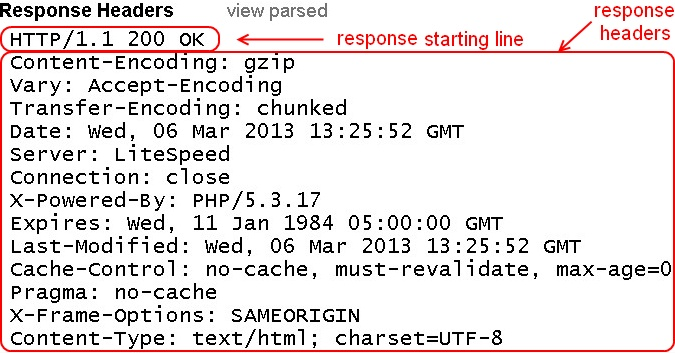
\includegraphics[width=\linewidth]{testimage}
\end{figure}

\subsection{Gra PONG wyświetlana na zdalnym monitorze}

System gry PONG dla dwóch graczy z możliwością kolejkowania chętnych złożony jest z trzech części:

\begin{enumerate}
  \item \textbf{Klienta webowego} w postaci strony internetowej uruchamianej na w przeglądarce internetowej na urządzeniu mobilnym użytkownika końcowego. Podobnie, jak w przypadku systemu pilota do sterowania zdalnym monitorem, klient ma za zadanie zapewnić komunikację, przechwytywać gesty wykonane na urządzeniu mobilnym oraz wyświetlać komunikaty i przyciski w zależności od stanu gry.
  \item \textbf{Serwera} obsługującego protokół Web Socket, który ma za zadanie obsługę połączeń klientów webowych, kolejkowanie ich zgłoszeń do gry, oraz uruchomienie gry na kliencie wyświetlającego grę. Serwer komunikuje się z klientem wyświetlającym grę za pomocą Web Socket, jako, że jest napisany jako aplikacja uruchamiana w przeglądarce internetowej.
  \item \textbf{Klient wyświetlający grę} - aplikacja stworzona jako strona internetowa uruchamiana w przeglądarce na ekranie LED. Wyświetla planszę gry w trakcie jej trwania, lub komunikaty zachęcające do podjęcia rozgrywki w trakcie, gdy nie trwa rozgrywka. Na ekranie można wyświetlać potencjalne reklamy.
\end{enumerate}

\subsubsection{Diagram komponentów}

\begin{figure}[h!]
  \caption{A picture of a gull.}
  \centering
    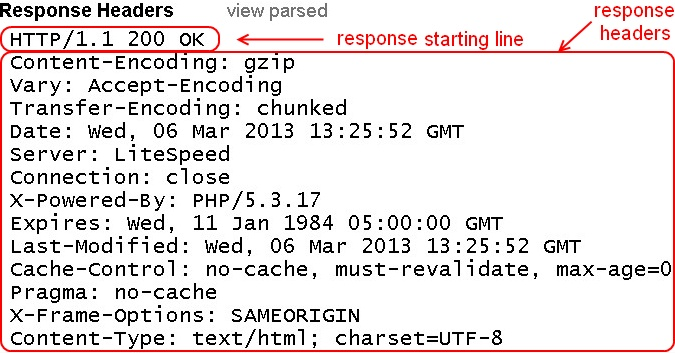
\includegraphics[width=\linewidth]{testimage}
\end{figure}

\subsubsection{Diagram interackji}

\begin{figure}[h!]
  \caption{A picture of a gull.}
  \centering
    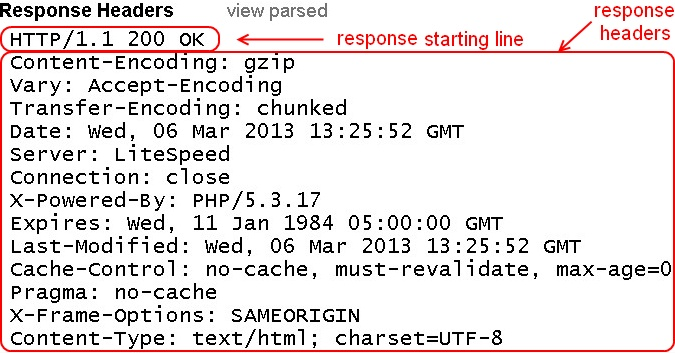
\includegraphics[width=\linewidth]{testimage}
\end{figure}
